\documentclass[10pt,twocolumn]{witseiepaper}

%==========================
\usepackage{KJN}
\usepackage{chngcntr}
\usepackage{multicol}
\usepackage[utf8]{inputenc}
\usepackage[TS1,T1]{fontenc}
\usepackage{array, booktabs}
\usepackage{graphicx}
\usepackage[x11names]{xcolor}
\usepackage{colortbl}
\usepackage{caption}
%==========================
\newcommand{\foo}{\makebox[0pt]{\textbullet}\hskip-0.5pt\vrule width 1pt\hspace{\labelsep}}

\ifpdf
\pdfinfo{
/Title (ELEN4002/ELEN4012 - Automatic Detection, Classification and Demodulation of Radio Signals)
/Author (Anthony Farquharson with Jacques Visser)
}
\fi

\begin{document}

\title{ELEN4002/ELEN4012 - Automatic Detection, Classification and Demodulation of Radio Signals}

\author{Anthony Farquharson (563648) \textnormal{\newline With: Jacques Visser (457817)
\newline Supervisor: Dr. Jaco Versfeld}
\thanks{School of Electrical \& Information Engineering, University of the
Witwatersrand, Private Bag 3, 2050, Johannesburg, South Africa}
}

\abstract{Automatic Modulation Classification is used to identify an unknown modulation scheme of a received signal. This report gives a preliminary breakdown of the development of an automatic modulation classification system, using the Universal Software Radio Peripheral. Various types of modulation classification techniques are discussed, and a Spectral-Based Feature classification technique is chosen. The design and implementation techniques are discussed, as well as a proposed project time line.}

\keywords{Classification, Modulation, USRP, UHD}

\maketitle
\thispagestyle{empty}\pagestyle{empty}

% TODO How does one even write an introduction?
\section{INTRODUCTION}
This preliminary report gives the design breakdown for an Automatic Modulation Classification (AMC) system, using the Ettus Research Universal Software Radio Peripheral (USRP) in conjunction with the USRP Hardware Driver (UHD) to identify radio signals.\\[10pt]
The system is designed to use the C++ programming language to implement a Spectral feature-based classifier, using K-Nearest Neighbor (KNN) classification. If time allows then a distribution-test based classifier will be implemented in conjunction with the feature-based classifier to improve results.\\[10pt]
A full description of the design and implementation techniques is given, describing the incremental design model. Trello is suggested to help manage the development process.\\[10pt]
A description of all recommended software tools for implementation is given, along with a full testing plan for production. The testing plan allows for the training of the KNN classifier. Preliminary results are presented using the Spectral Feature-based classification technique, along with reasons to use the KNN classifier.

\section{LITERATURE SURVEY}
\label{sec:literature}
According to Zhu and Nandi \cite{zhu2014automatic} there are three primary approaches to automatic modulation classification (AMC), these are: likelyhood-based, distribution-test-based and feature based. These will be discussed briefly below.

	\subsection{Likelihood Based Classification}
	\label{subsec:likelyhood}
	Likelihood based classification is the considered the most popular method of classification, due to the accuracy of the classification when the channel is perfectly modeled \cite{zhu2014automatic}. This method requires knowledge of the channel that the signal is received from, which can be derived through evaluating every modulation hypothesis with observed signal samples \cite{zhu2014automatic}.\\[10pt]

	The main likelihood based classifier approaches are as follows \cite{zhu2014automatic}:
	\begin{itemize}
		\item \textbf{Maximum Likelihood (ML)} - This classifier requires perfect channel knowledge and all parameters are known except for the signal modulation.
		\item \textbf{Average Likelihood Ratio Test (ALRT)} - This classifier overcomes the limitation of not knowing every parameter through using accurate models for unknown parameters, making the calculation much more complex when unknown parameters are introduced.
		\item \textbf{Generalized Likelihood Ratio Test (GLRT)} - Essentially a combination of ALRT and ML classifiers, it replaces the integration of unknown parameters (ALRT) with maximization of likelihood for a possible range of unknown parameters.
		\item \textbf{Hybrid Likelihood Ratio Test (HLRT)} - The HLRT likelihood function is calculated by averaging transmitted symbols and maximizing the resulting function.
	\end{itemize}
	These classifiers are well documented by Zhu and Nandi \cite{zhu2014automatic}; and Dobre, Abdi, Bar-Ness and Su \cite{dobre2007survey}. 

	\subsection{Distribution Test Based Classification}
	\label{subsec:distribution}
	
	The distribution test based classification uses the symbol mapping, which is associated with a particular modulation scheme. This is assuming that the channel parameters are pre-estimated and available \cite{zhu2014automatic}.
	
	The technique uses a method known as ``Goodness of Fit'' which will equate the differences between known signal cumulative distributions and the received signal cumulative distribution. The classification is completed by finding the signal distribution with the best goodness of fit \cite{zhu2014automatic}.
	
	There are many distribution tests which can be used to evaluate the goodness of fit, some of them are given below \cite{zhu2014automatic}:
	\begin{itemize}
		\item \textbf{Kolmogorov-Smirnov Test Classifier} - This goodness of fit test evaluates the equality of two probability distributions, for the classifier the sampled cumulative distribution function (CDF) and a hypothesized CDF are considered.
		\item \textbf{Cramer-Von Mises Test Classifier} - The method of the classifier is the same as the Kolmogorov-Smirnov classifier, but the goodness of fit criterion is different.
		\item \textbf{Anderson-Darling Test Classifier} - This classifier uses a weighted version of the Cramer-Von Mises test classifier. The tail of the distribution is weighted to counter the fact that it converges to zero at that point.
	\end{itemize}
	The distribution test based classifiers are well documented by Zhu and Nandi \cite{zhu2014automatic}; and Dobre, Abdi, Bar-Ness and Su \cite{dobre2007survey}.

	\subsection{Feature Based Classification}
	\label{subsec:feature}
	
	The feature based modulation classification is shown to not be as accurate, but is significantly less computationally intensive than the Distribution test based and likelihood based classifiers \cite{zhu2014automatic}.
	
	The feature based classification technique uses the primary features of a signal in order to classify it as a particular modulation scheme. The features that are primarily used to identify the signal vary depending on the method employed.
	
	The main methods of feature based classification are as follows \cite{zhu2014automatic}: 
	\begin{itemize}
		\item \textbf{Signal Spectral-Based Features} - The key features of a signal analyzed by this technique exploit the three primary signal aspects, namely the amplitude, phase and frequency. This technique is well documented by Azzouz and Nandi \cite{azzouz2013automatic}.
		\item \textbf{Wavelet Transform-based Features} - This classification technique uses a continues wavelet transform of a received signal in order to determine the type of modulation used, using known criterion for various modulation features.
		\item \textbf{High-order Statistics-based Features} - The statistics based classification technique can use moment based and cumulative based features in order to determine which modulation scheme is used on the signal.
	\end{itemize}
	The distribution test based classifiers are well documented by Zhu and Nandi \cite{zhu2014automatic}; Azzouz and Nandi \cite{azzouz2013automatic}; and Dobre, Abdi, Bar-Ness and Su \cite{dobre2007survey}.

\section{EXISTING SOLUTIONS AND APPLICATIONS OF AMC}
	\subsection{Military Applications}
		Automatic modulation classification can be used in a variety of milatary applications, including Electronic Attack, Electronic Support and Electronic Protect \cite{zhu2014automatic}.\\[10pt]
		In Electronic attack the AMC system could be used to identify the modulation scheme of a signal that should be jammed. Once this has been identified the signal jamming can be done in such a way that it does not interfere with other signals, and does not waste power \cite{zhu2014automatic}.
	\subsection{Civilian Applications}
		The automatic modulation classification can be used in a link adaptation system. Depending on the channel noise, the modulation scheme could be changed in order to maintain maximum reliability in a noisy channel and maximum throughput in a clear channel \cite{zhu2014automatic}. Thus the use of adaptive modulation ensures that the link is optimal in any channel situation.

\section{SOLUTION SELECTION}
Of the three major types of modulation classification discussed in Section \ref{sec:literature} above, the method chosen for the purposes of this project is Spectral Feature-Based Modulation classification. This is motivated by the relative efficiency of the method (compared to the other two methods) \cite{zhu2014automatic} and the fact that a lot of previous work has been done on this method.\\[10pt]
The algorithm could be extended to attempt to incorporate distribution test-based classification techniques if time allows. These techniques could allow for a wider range of digital signals to be classified. The K-Nearest neighbor classifier (See section \ref{subsec:classifier}) could be extended to use the distribution goodness of fit value as an additional feature, which could expand the range of results.

\section{DESIGN PROCESS OVERVIEW}
	Automated modulation classification is primarily a software orientated problem, therefore a good development methodology must be laid out. In order to ensure quality of software output the following development methodologies are used.
	\subsection{Development Methodology}
	\label{subsec:devmethod}
	The development methodology chosen for this project is the Incremental Model, this model allows for a continuous use of small waterfall type development cycles \cite{incremental_model}. This methodology is chosen because the waterfall cycles allow for every iteration to be tested and integrated into the main project, reducing the chances of errors. \\[10pt]
	In order to track the various incremental cycles a Kanban approach \cite{kanban_model} will be used, this method uses a ``billboard'' of tasks, each task on the board will make up a small waterfall development cycle. These tasks will be tracked through use of Trello \cite{trello}, and every task will go through the stages from ``Pending'' to ``In Progress'' and finally ``Completed''.	
	
\section{PROJECT TIMELINE}
For the project duration the tasks are broken up into clear phases, starting with the software development, which includes the iterative development methodology (see Section \ref{subsec:devmethod}). Through this phase continuous unit and integration testing occurs.\\[10pt]
The next phase is the where framework testing and classifier training begins, for this a mocking technique will be used to imitate the UHD API and test the classifier. \\[10pt]
The following phase includes the real world testing and documentation, this section is where the system is tested under real world conditions through use of the USRP. Documentation can be generated during this phase.\\[10pt]
The last few phases are dedicated to the inspection of the project and generating the documentation and final reports, finally leading up to the final submission of the report.
\begin{table}[h]
    \renewcommand\arraystretch{1.4}
    \captionsetup{singlelinecheck=false, labelsep=quad}
    \caption{Timeline of Major Events in the Project Development}\vskip -1.5ex
    \begin{tabular}{@{\,}r <{\hskip 2pt} !{\foo} >{\raggedright\arraybackslash}p{6cm}}
    \toprule
    \addlinespace[1.5ex]
    09-07 & Project Begins, Development of Software Framework Starts\\
    09-21 & Framework Development Complete, Framework Testing and Classifier Training Starts\\
    09-28 & Real-World Testing and Documentation\\
    10-14 & Project inspection\\
    10-19 & Documentation\\
    10-23 & Submission of final report\\
    \end{tabular}
    \label{tab:time}
\end{table}

\section{IMPLEMENTATION OVERVIEW}
	\subsection{Hardware}
		The implementation will use a software defined radio, specifically the Universal Software Radio Peripheral (USRP) from Ettus Research \cite{ettus}. The USRP Hardware Driver (UHD) interfaces the software with the hardware system, due to lack of support for Windows this means the development will be done on Linux platforms.

	\subsection{Software}
	The UHD has an application programming interface (API) for use with the C++ programming language, allowing the development to be done in C++.
		\subsubsection{Basic Software Structure}
			As the algorithm should be ideally running in a real-time situation, the efficiency becomes a priority. For this reason the program will be threaded to allow for concurrent processes, this means that every major component will run on it's own thread.\\[10pt]
			The algorithm will separate the various processes out into their categories, allowing for a good layer separation. This means that components can be individually modified, replaced or mocked for testing. The program will run around a primary control loop, where information will be read from the UHD buffer, then processed (see Figure \ref{fig:sw_overview} below) and finally displayed. The feature extraction component is fully explored in Section \ref{subsec:feature_extract} below, and a full layout is given in Figure \ref{fig:feature} Appendix \ref{app:feature}.
			\begin{figure}[h!]
				\centering
				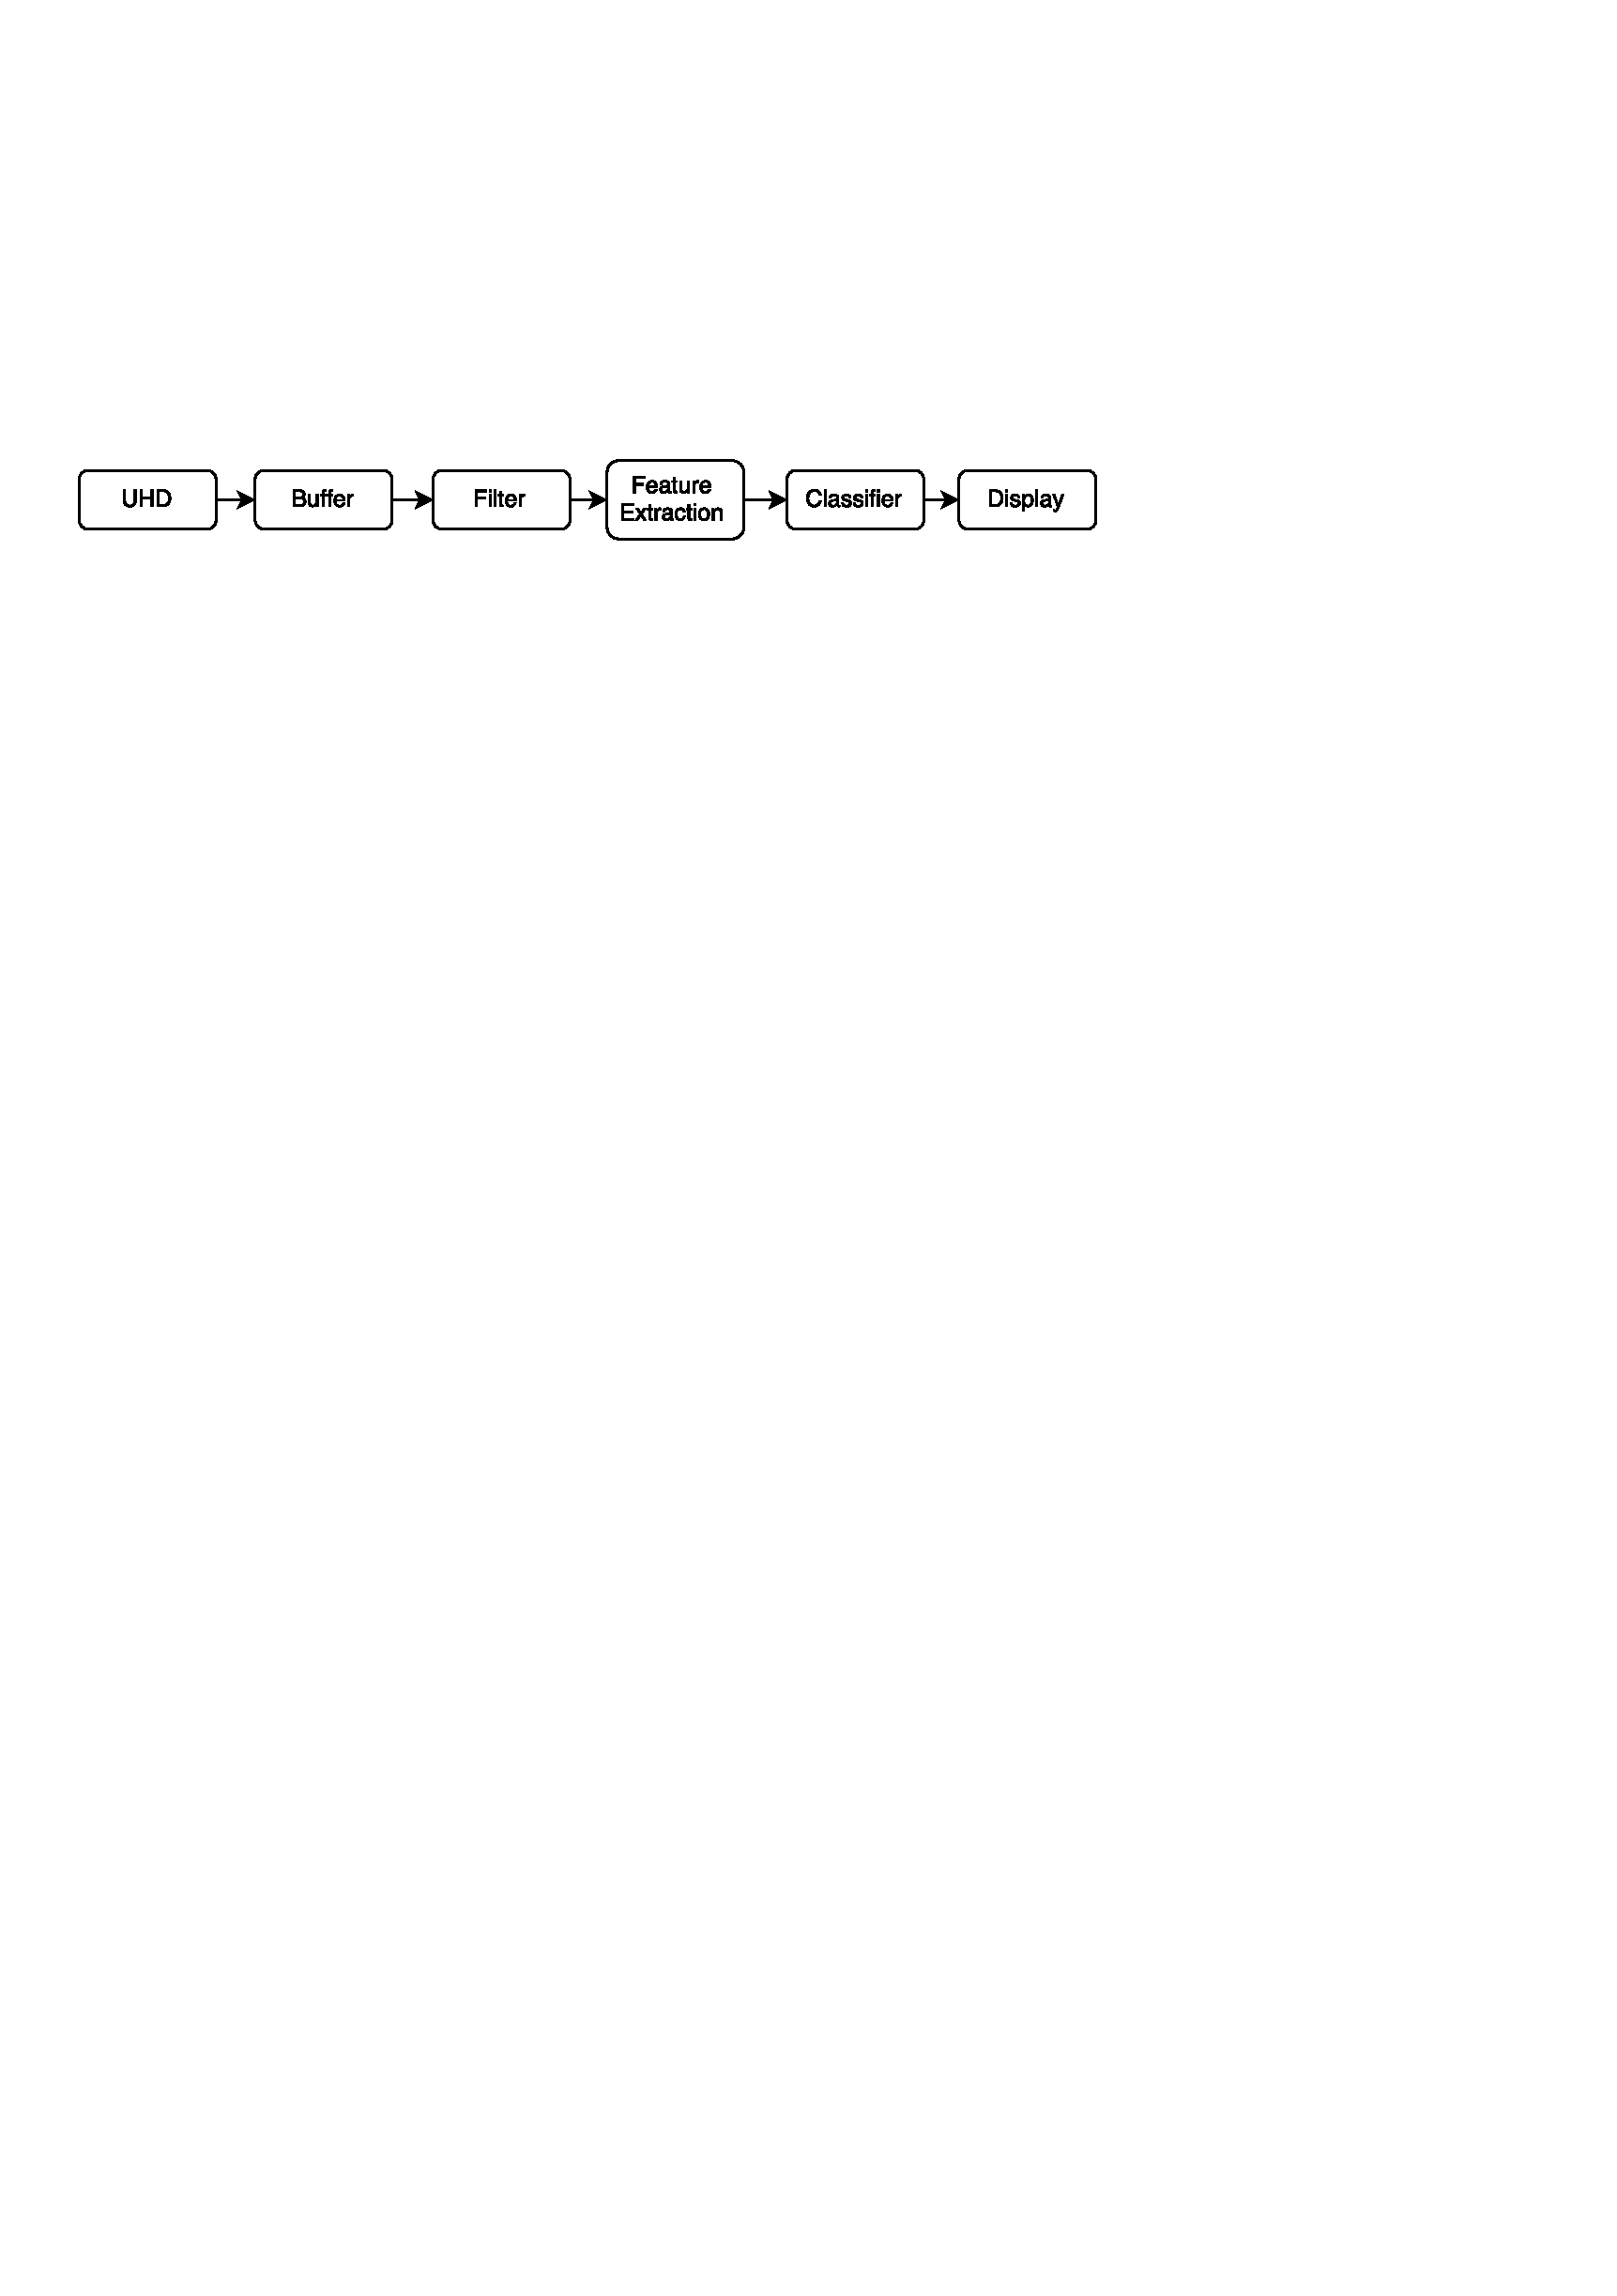
\includegraphics[trim=1.2cm 31.5cm 9cm 8cm, clip=true,width=0.5\textwidth]{small.pdf}
				\caption{Modulation Classification Algorithm Overview.}
				\label{fig:sw_overview}
			\end{figure}
		\subsubsection{Libraries and API's}
			The nature of the software implementation is very complex, meaning that developing every component would be out of the scope of the project. To account for this several programming libraries and API's are used, these are discussed below in the order that they are processed in Figure \ref{fig:sw_overview}.\\[10pt]
			The first component is the USRP Hardware Driver (UHD), this interfaces the USRP device with the program through the use of an API. The UHD is licensed under Gnu Public License version 3 (GPLv3) \cite{uhd_license}, which allows free and open source use for the purposes of this project.\\[10pt]
			The UHD programming interface is designed to be used with the C++ programming language. The C++11 standard has a multitude of libraries and tools that are useful in the context of this project. This makes it the ideal platform to build the program on. The C++11 standard library is licensed under GPLv3 for free and open-source use.\\[10pt]
			One of the primary operations on the signal is to get the frequency components, which involves the use of a Fast Fourier Transform (FFT). To this end the FFTW3 library is used. The FFTW3 library is an efficient, open-source library licensed under GPLv3 \cite{fftw3_license}.\\[10pt]
			In order to display relevant information the QT framework is to be used, as it is a well documented and widely used display framework. The QT framework has a variety of useful display tools (widgets) such as QCustomPlot, which can be used in the display of graphs and plots. For convenient testing the QT Testing framework will also be used during the development process. These frameworks are licensed under GPLv3.
			
		\subsubsection{Build System}
			As a variety of libraries and tools need to be used in conjunction, a build tool must be used to compile everything together. To serve this purpose the CMake build tool is to be used, as it is well documented and widely used. This allows for a well supported and easy to use build system, which can compile to multiple platforms. \\
			Cmake is licensed under the BSD 3-Clause license \cite{cmake_license}, allowing for use in this project.

	\subsection{Feature Extraction Functions}
	\label{subsec:feature_extract}
	The individual features of the signal must be extracted, so that they can be used in the classifier to determine the modulation technique. The features to be extracted are shown in Appendix \ref{app:feature}. As some of the feature extraction techniques have an overlap of data, the process can be optimized by only computing the necessary components once, for more see Figure \ref{fig:feature}.\\[10pt]
	A major part of the feature extraction requires spectral analysis, thus a Fourier function must be derived from the input signal. The Fourier transform is computed using the FFT function in the FFTW3 library.\\[10pt]
	The instantaneous phase can be determined through spectral analysis as well, by taking the signal's Fourier function (determined by FFT) and removing the negative components of the signal. This transforms the signal into a complex signal, this is obtained by taking an inverse fast Fourier transform (IFFT) of the modified Fourier function, then phase unwrapping must be performed \cite{zhu2014automatic,azzouz2013automatic}. Once the instantaneous phase has been determined the instantaneous frequency can be derived through differentiation. \\[10pt]

	\subsection{Signal Filtering}
	Signal filtering is vitally important, as it is required to isolate the bandwidth in which the signal exists. This filtering will be done through a digital filter, independent of the USRP. The filter must not interfere with the phase of the signal, as some of the features are dependent on the non-linear portion of the phase. To this end zero-phase digital filtering must be implemented, by either selecting a Finite Impulse Response (FIR) filter or by forward and reverse filtering an Infinite Impulse Response (IIR) filter.\\[10pt]
	There are downsides and benefits to both zero-phase filtering techniques, and thus the type of filter to be used is still under consideration. In implementation both filters my be tested and the better performing filter selected for use.\\[10pt]
	The implementation of the filter can be done in two ways, either by multiplication within the Fourier domain, or by convolution of the signal in the time domain. Using the Fourier domain technique would result in an additional step in the feature extraction, see Appendix \ref{app:feature} for more.

	\subsection{Classifier}
	\label{subsec:classifier}
	The classifier selected for this application is the K-Nearest neighbor, which analyzes the number of nearest reference signals in the feature space. This technique uses the fact that the features from the same modulation schemes will group together in the feature space. K-Nearest neighbor has three main steps, which are as follows \cite{zhu2014automatic}:
	\begin{enumerate}
		\item \textbf{Reference Feature Space} - The feature space will contain M reference values for each of the features, the value of M is calculated heuristically. 
		\item \textbf{Distance Definition} - The distance definition can be completed through a Euclidean distance function between feature sets, in order to calculate the distances between them.
		\item \textbf{K-Nearest Neighbor Decision} - Once all distances have been calculated, a number of k reference signals are recorded as the k nearest neighbors. k must be determined through a set of rules, and can be optimized.
	\end{enumerate}
	This classifier must be trained in order to work, so many simulations must be run to build up the reference pool of neighbors. The training occurs during the first step in the design process, where the reference feature space is built \cite{zhu2014automatic}.

\section{PROPOSED TESTING PROCEDURE}
	The software testing will be completed through the use of a unit testing framework, for this the QtTest framework has been selected. The primary reason being that the QT framework is already in use for display, so additional unnecessary libraries will not need to be installed. The functional testing will serve to train the classifier by feeding in test signals and building the feature space. The practical testing will feed the classifier realistic signals once it has been trained in order to evaluate the effectiveness.
	\subsection{Preliminary Testing}
		Preliminary testing will be performed on the UHD API, this important step will show that the various tools selected will work together realistically. A simple example code from the Ettus website \cite{uhd_tutorial} will be used in conjunction with the USRP to test the API.
	\subsection{Functional Testing}
		The functional testing will be done through use of a mocking framework. The mocking framework will emulate the UHD API in testing, and feed the classifier testing signals. This technique will allow the classifier to be trained with a variety of expected signals. This step will also give useful information on the performance of the system.
	\subsection{Practical Testing}
		The practical testing can only be completed once the classifier has been trained. This testing will use the actual USRP and UHD in order to realistically test the modulation classification over a non-ideal channel. This step will evaluate the accuracy of the feature-based modulation classification scheme.
\section{PRELIMINARY RESULTS}
	A limited feature-based modulation classification algorithm was performed in MATLAB, the results show the clear separation of different modulation schemes even with the limited amount of features. The results of this can be seen in Figure \ref{fig:prelim} Appendix \ref{app:prelim}.\\[10pt]
	The implementation of a threshold-based decision-tree classifier showed that the technique was possible and would indeed work. However this method of classification requires a large amount of application logic to sort through the possibilities, and thus is not particularly extensible. This is why the K-Nearest Neighbor method of classification was selected, as it allows for the classifier to be ``Trained'' for relevant modulation schemes.
\section{CONCLUSION}
This proposal presented an Automatic Modulation Classification design using the USRP to implement a Spectral Feature-based classifier. The design incorporates the use of a K-Nearest Neighbor classification technique and various software and organizational tools required for a project of this scope. \\[10pt]
A full description of the project timeline as well as software development techniques to organize the project are presented, with a plan to test and train the KNN classifier. A full breakdown of required signal analysis techniques is given, as well as the tools required in implementation of these techniques.

\bibliographystyle{witseie}
\bibliography{prelim}
\newpage

\onecolumn
\appendix
\counterwithin{figure}{section}
\section{Feature Extraction Process}
\label{app:feature}
Feature extraction is a relatively complex process, but has a lot of room for optimization as the compartmental nature of the different features allows for a certain amount of threading. This threading can be achieved using the C++11 standard threading library.\\[11pt]
The features presented in Figure \ref{fig:feature} below are those documented by Zhu and Nandi \cite{zhu2014automatic}, as well as Azzouz and Nandi \cite{azzouz2013automatic}. The features are as follows: 
\begin{itemize}
	\item $\gamma_{max}$ - Maximum value of Power Spectral Density.
	\item $\sigma_{ap}$ - Standard Deviation of the Absolute value of the non-linear component of instantaneous phase.
	\item $\sigma_{dp}$ - Standard Deviation of the non-linear component of direct instantaneous phase.
	\item $P$ - Spectral Symmetry.
	\item $\sigma_{aa}$ - Standard Deviation of the Absolute value of the normalized and centered instantaneous amplitude.
	\item $\sigma_{af}$ - Standard Deviation of the absolute value of the normalized and centered instantaneous frequency.
	\item $\sigma_{a}$ - Standard Deviation of the normalized and centered instantaneous amplitude.
	\item $\mu_{42}^{a}$ - Kurtosis of the normalized and centered instantaneous amplitude.
	\item $\mu_{42}^{f}$ - Kurtosis of the normalized and centered instantaneous frequency.
\end{itemize}

\begin{figure}[h!]
	\centering
	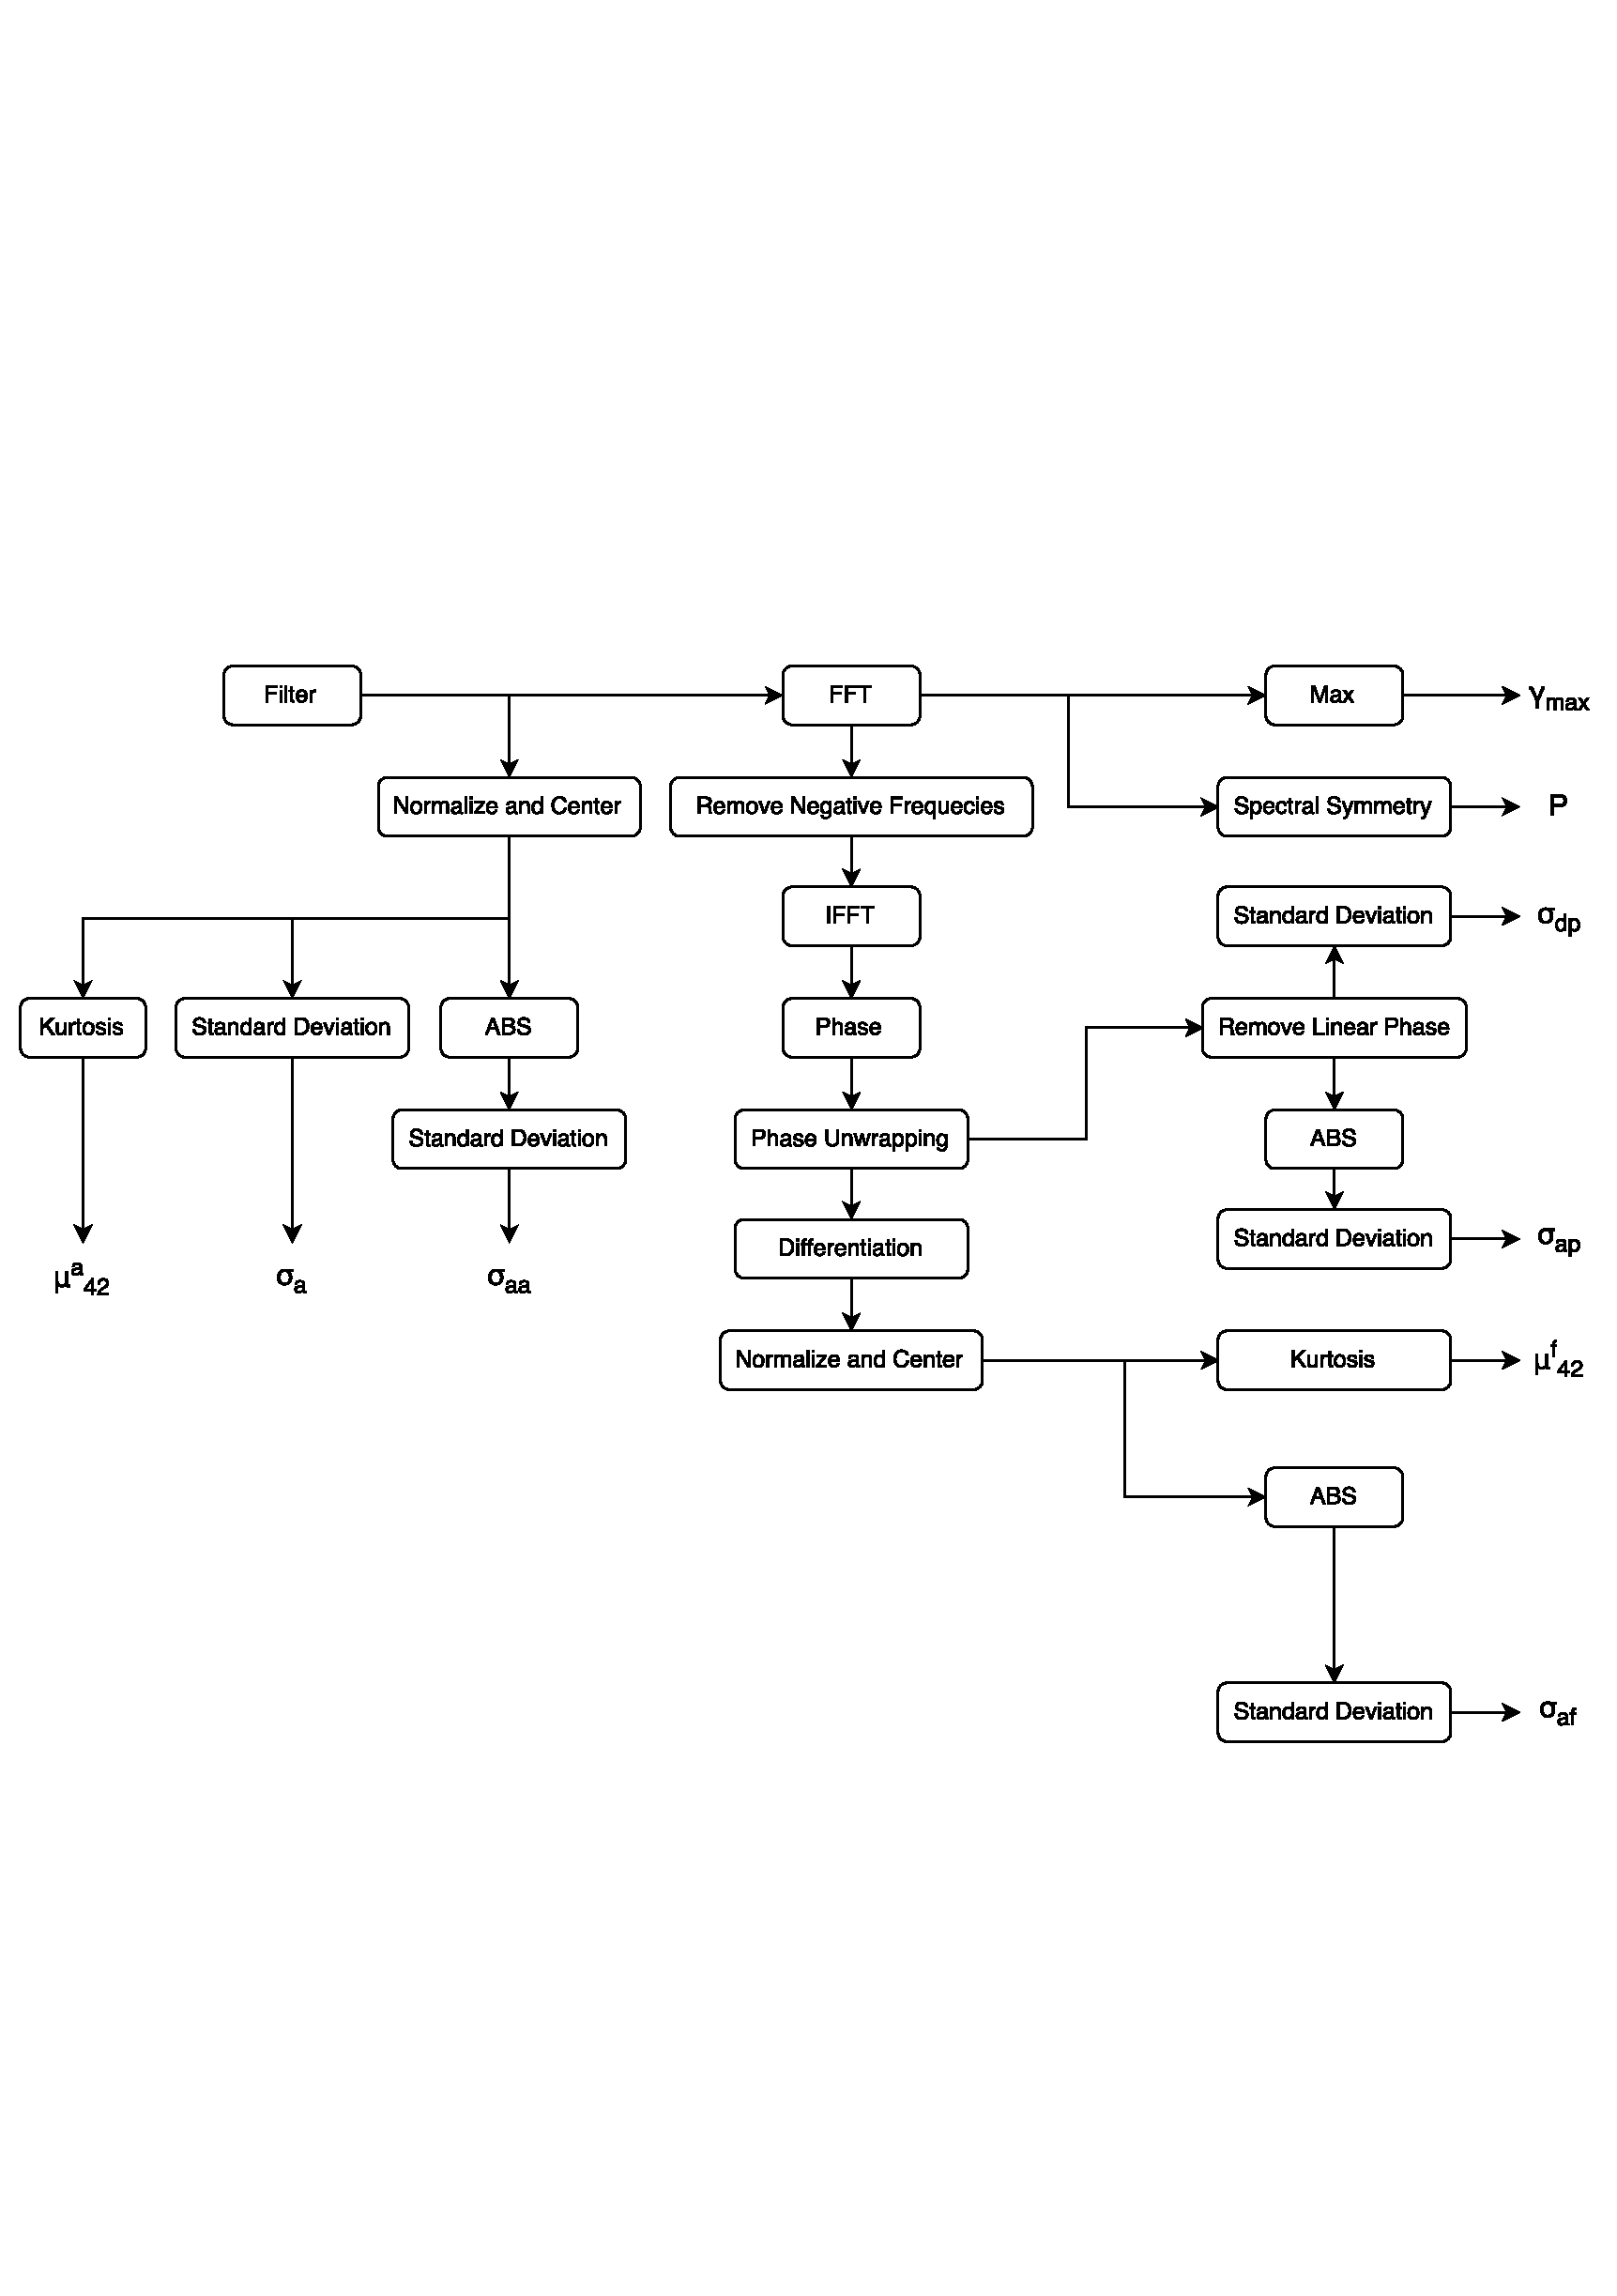
\includegraphics[trim=0cm 10cm 0cm 11cm, clip=true,width=0.8\textwidth]{large.pdf}
	\caption{Feature extraction process as a flow chart}
	\label{fig:feature}
\end{figure}

\newpage
\section{Preliminary Results}
\label{app:prelim}
Figure \ref{fig:prelim} below shows the resulting limited features of various input signals to a preliminary testing function. The signals included modulated music with Gaussian noise introduced, as well as real world AM and FM signals.
\begin{figure}[!h]
	\centering
	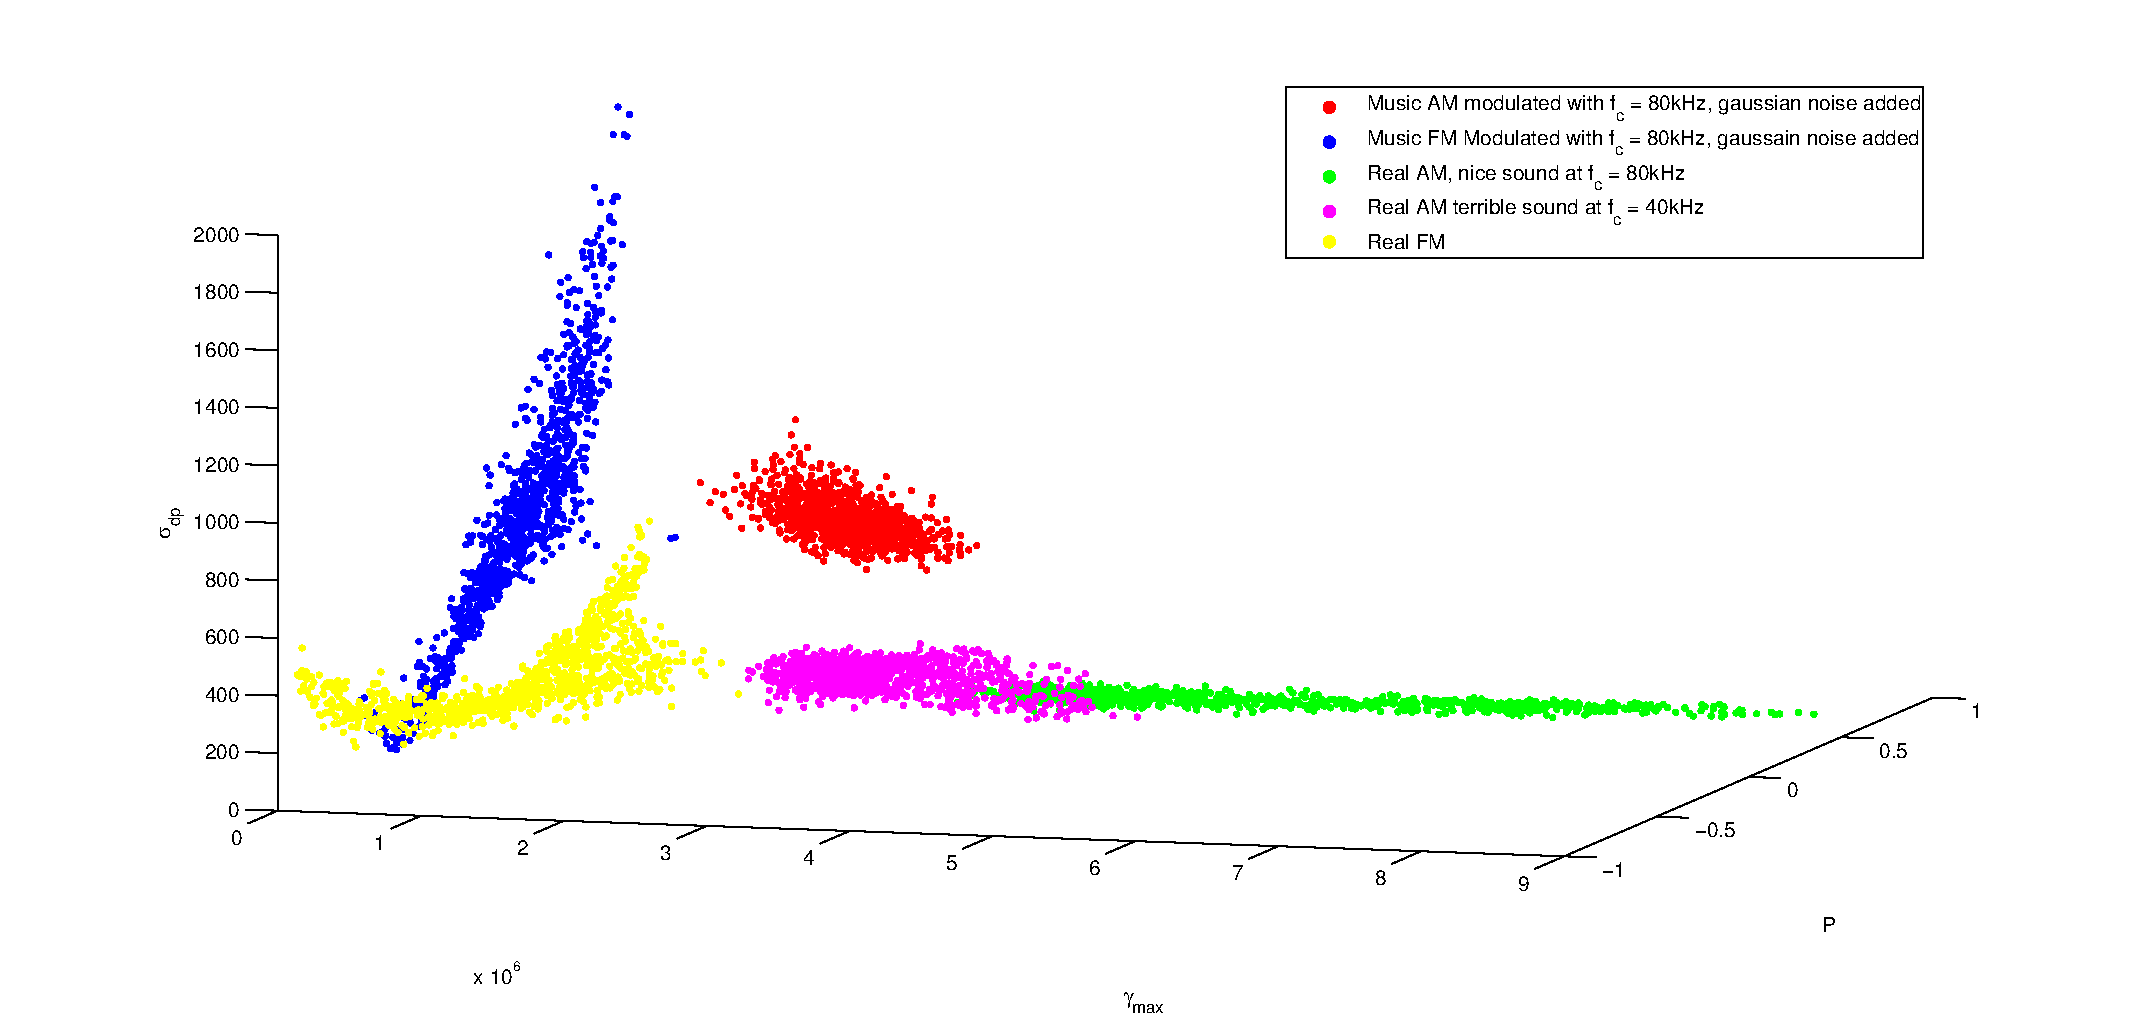
\includegraphics[width=1.1\textwidth]{plot0-eps-converted-to.pdf}
	\caption{Plot of $\sigma_{dp}$ vs. $\gamma_{max}$ vs. $P$ for various AM and FM signals}
	\label{fig:prelim}
\end{figure}

\end{document}
